\documentclass[a4paper,14pt]{extarticle}
\usepackage[utf8]{inputenc}
\usepackage[T2A]{fontenc}
\usepackage[russian]{babel}
\usepackage{geometry}
\usepackage{graphicx}
\usepackage{array}
\usepackage{longtable}
\usepackage{titlesec}
\usepackage{hyperref}
\usepackage{setspace}
\usepackage{indentfirst}
\usepackage{fancyhdr}
\usepackage{amsmath,amssymb}
\usepackage{listings}
\usepackage{xcolor}
\usepackage{multirow}

\geometry{left=3cm, right=1.5cm, top=2cm, bottom=2cm}
\onehalfspacing
\setlength{\parindent}{1.25cm}

\pagestyle{fancy}
\fancyhf{}
\fancyfoot[C]{\thepage}
\renewcommand{\headrulewidth}{0pt}

\titleformat{\section}[block]{\normalfont\bfseries\centering}{\thesection}{0.5em}{}
\titleformat{\subsection}[block]{\normalfont\bfseries}{\thesubsection}{0.5em}{}

\definecolor{codebg}{rgb}{0.96,0.96,0.96}
\lstdefinestyle{py}{
    language=Python,
    backgroundcolor=\color{codebg},
    basicstyle=\ttfamily\small,
    keywordstyle=\color{blue},
    commentstyle=\color{gray},
    stringstyle=\color{teal},
    numbers=left,
    numberstyle=\tiny,
    breaklines=true,
    frame=single,
    tabsize=4,
    showstringspaces=false,
}

\begin{document}

% ========== ТИТУЛЬНЫЙ ЛИСТ ==========
\begin{titlepage}
\begin{center}


\includegraphics[width=1.2cm]{images/logo.jpg}

\smallskip
\small
МИНИСТЕРСТВО НАУКИ И ВЫСШЕГО ОБРАЗОВАНИЯ РОССИЙСКОЙ ФЕДЕРАЦИИ

\smallskip
Федеральное государственное автономное образовательное учреждение высшего образования

\smallskip
\textbf{<<Дальневосточный федеральный университет>>}

\textbf{(ДВФУ)}

\vspace{5mm}
\noindent\rule{\textwidth}{2pt}

\vspace{10mm}
{\large\textbf{ИНСТИТУТ МАТЕМАТИКИ И КОМПЬЮТЕРНЫХ ТЕХНОЛОГИЙ}}

\vspace{5mm}
\textbf{Департамент математического и компьютерного моделирования}

\vspace{15mm}
Избосарова Жасмина Олимжоновна

\vspace{5mm}
{\large\textbf{МЕТОД ПРОСТОЙ ИТЕРАЦИИ ДЛЯ РЕШЕНИЯ\\ УРАВНЕНИЯ ВОЛЬТЕРРА 2 РОДА}}

\vspace{10mm}
{\large\textbf{КУРСОВОЙ ПРОЕКТ}}

\vspace{5mm}
Студентка группы Б9123-02.03.01сцт

\vspace{3mm}
Руководитель \_\_\_\_\_\_\_\_\_\_\_\_\_\_\_\_\_\_\_\_

\end{center}

\vspace{10mm}

\noindent Регистрационный № \_\_\_\_\_\_\_\_\_\_\_ \hfill Оценка \_\_\_\_\_\_\_\_\_\_\_\_\_\_\_\_\_\_\_\_\_\_

\vspace{10mm}

\noindent\makebox[7cm]{\hrulefill} \hfill \makebox[7cm]{\hrulefill}

\noindent\makebox[7cm][c]{\footnotesize (подпись)\hspace{2cm}(И.\,О.\,Фамилия)} \hfill
\makebox[7cm][c]{\footnotesize (подпись)\hspace{2cm}(И.\,О.\,Фамилия)}

\vspace{5mm}

\noindent\makebox[7cm][c]{\footnotesize <<\_\_\_>> \_\_\_\_\_\_\_\_\_\_\_\_\_\_\_\_ 2026 г.} \hfill
\makebox[7cm][c]{\footnotesize <<\_\_\_>> \_\_\_\_\_\_\_\_\_\_\_\_\_\_\_\_ 2026 г.}

\vfill

\begin{center}
г. Владивосток\\
2026
\end{center}

\end{titlepage}

% ========== СОДЕРЖАНИЕ ==========
\tableofcontents
\newpage

% ========== ВВЕДЕНИЕ ==========
\section*{Введение}
\addcontentsline{toc}{section}{Введение}

Интегральные уравнения Вольтерра второго рода возникают во многих прикладных задачах: в теории восстановления, в задачах с памятью (вязкоупругость, демография, эпидемиология), при сведении задачи Коши для обыкновенных дифференциальных уравнений к эквивалентной интегральной форме, в теории автоматического регулирования и в ряде других разделов математической физики. В отличие от уравнений Фредгольма, уравнения Вольтерра обладают важным свойством: верхний предел интегрирования зависит от переменной $x$, вследствие чего соответствующий интегральный оператор является <<вольтерровым>> (квазинильпотентным), что обеспечивает безусловную сходимость метода последовательных приближений при любом значении параметра $\lambda$ --- в этом состоит принципиальное отличие от уравнений Фредгольма, где сходимость метода простой итерации требует выполнения условия $|\lambda| \cdot M (b-a) < 1$.

Целью курсового проекта является изучение теоретических основ метода простой итерации для линейного интегрального уравнения Вольтерра второго рода, построение вычислительной схемы на основе квадратурных формул, программная реализация алгоритма и проведение численного эксперимента с оценкой точности и порядка сходимости.

Для достижения цели поставлены следующие задачи:
\begin{enumerate}
\item рассмотреть постановку задачи и теоретические основы метода последовательных приближений (метода простой итерации) для уравнения Вольтерра II рода;
\item обосновать безусловную сходимость метода и получить оценку скорости сходимости;
\item построить вычислительную схему, сочетающую метод простой итерации с квадратурной формулой трапеций для дискретизации интеграла;
\item реализовать алгоритм на языке Python;
\item провести вычислительный эксперимент на тестовых примерах с известным точным решением, исследовать зависимость погрешности от шага сетки и от номера итерации;
\item сформулировать выводы по результатам работы.
\end{enumerate}

Постановка задачи соответствует методическому указанию~[2, с.~71].

% ========== ГЛАВА 1 ==========
\section{Теоретические основы метода простой итерации}

\subsection{Постановка задачи}

Рассматривается линейное интегральное уравнение Вольтерра второго рода относительно неизвестной функции $y(x)$:
\begin{equation}
y(x) = f(x) + \lambda \int_{a}^{x} K(x,s)\, y(s)\, ds, \qquad x \in [a,b],
\label{eq:volterra}
\end{equation}
где $f(x)$ --- заданная непрерывная на $[a,b]$ функция, $K(x,s)$ --- ядро уравнения, непрерывное в треугольнике $a \le s \le x \le b$, $\lambda$ --- числовой параметр. В отличие от уравнения Фредгольма второго рода, верхний предел интегрирования в~\eqref{eq:volterra} совпадает с переменной $x$, что делает оператор
\[
(A y)(x) = \int_a^x K(x,s)\, y(s)\, ds
\]
вольтерровым: его спектральный радиус равен нулю при любом непрерывном ядре $K$.

\subsection{Метод последовательных приближений (метод простой итерации)}

Метод простой итерации (метод последовательных приближений Пикара) состоит в построении последовательности функций $y_0(x), y_1(x), y_2(x), \dots$ по правилу
\begin{equation}
y_0(x) = f(x), \qquad
y_{n+1}(x) = f(x) + \lambda \int_a^x K(x,s)\, y_n(s)\, ds, \qquad n = 0,1,2,\dots
\label{eq:picard}
\end{equation}

\textbf{Сходимость метода.} Пусть $|K(x,s)| \le M$ при $a \le s \le x \le b$. Тогда для разности двух последовательных приближений справедлива оценка
\[
|y_{n+1}(x) - y_n(x)| \le \frac{(|\lambda| M)^{n+1} (x-a)^{n+1}}{(n+1)!} \max_{[a,b]} |f|.
\]
Эта оценка получается по индукции: ядро $n$-й итерированной степени оператора $A$ оценивается величиной $\dfrac{M^n (x-s)^{n-1}}{(n-1)!}$, то есть убывает быстрее любой геометрической прогрессии за счёт факториала в знаменателе. Следовательно, ряд
\[
y(x) = y_0(x) + \sum_{n=0}^{\infty} \bigl(y_{n+1}(x) - y_n(x)\bigr)
\]
сходится равномерно на $[a,b]$ \emph{при любом} значении $\lambda$ и любом непрерывном ограниченном ядре $K$ --- в этом и состоит \textbf{безусловная сходимость} метода простой итерации для уравнения Вольтерра второго рода (теорема Марчука--Пикара, см.~[1]). Предельная функция $y(x) = \lim_{n\to\infty} y_n(x)$ является единственным непрерывным решением уравнения~\eqref{eq:volterra}.

Скорость сходимости метода, таким образом, факториальная: погрешность $n$-го приближения убывает как $\dfrac{(|\lambda|M(b-a))^n}{n!}$, что на практике означает достижение заданной точности за весьма небольшое число итераций (что подтверждается численным экспериментом в главе~3).

\subsection{Квадратурная формула для дискретизации интеграла}

Для численной реализации метода интеграл в~\eqref{eq:picard} заменяется составной квадратурной формулой трапеций. Введём равномерную сетку
\[
x_i = a + i h, \quad h = \frac{b-a}{N}, \quad i = 0,1,\dots,N.
\]
Тогда для каждого узла $x_i$
\begin{equation}
\int_a^{x_i} K(x_i,s)\, y(s)\, ds \approx h \sum_{j=0}^{i} c_{ij}\, K(x_i,x_j)\, y(x_j),
\qquad
c_{ij} =
\begin{cases}
1/2, & j = 0 \text{ или } j = i,\\
1, & 0 < j < i,
\end{cases}
\label{eq:quad}
\end{equation}
с погрешностью $O(h^2)$ на гладких $f$ и $K$.

\subsection{Вычислительная схема}

Объединяя~\eqref{eq:picard} и~\eqref{eq:quad}, получаем дискретный аналог метода простой итерации: обозначим $Y_i^{(n)} \approx y_n(x_i)$,
\begin{equation}
Y_i^{(0)} = f(x_i), \qquad
Y_i^{(n+1)} = f(x_i) + \lambda h \sum_{j=0}^{i} c_{ij}\, K(x_i,x_j)\, Y_j^{(n)}, \qquad i = 0,\dots,N.
\label{eq:scheme}
\end{equation}
Итерации по $n$ прекращаются при выполнении критерия остановки
\[
\max_{0 \le i \le N} \bigl| Y_i^{(n+1)} - Y_i^{(n)} \bigr| < \varepsilon
\]
для заданной точности $\varepsilon$. Таким образом, суммарная погрешность численного решения складывается из погрешности метода простой итерации (факториально убывающей по $n$) и погрешности квадратурной формулы трапеций (порядка $O(h^2)$ по шагу сетки).

% ========== ГЛАВА 2 ==========
\section{Программная реализация}

\subsection{Описание алгоритма}

Алгоритм реализован на языке Python с использованием библиотеки \texttt{numpy} для векторных вычислений и \texttt{matplotlib} для построения графиков. Основные шаги алгоритма:

\begin{enumerate}
\item построить равномерную сетку $x_0,\dots,x_N$ с шагом $h=(b-a)/N$;
\item вычислить вектор $F = (f(x_0),\dots,f(x_N))$ и положить $Y^{(0)} = F$;
\item на каждой итерации для каждого узла $x_i$ вычислить квадратурную сумму~\eqref{eq:quad} по формуле трапеций с весами $c_{ij}$ и получить новое приближение $Y^{(n+1)}$ по формуле~\eqref{eq:scheme};
\item вычислить невязку $\|Y^{(n+1)} - Y^{(n)}\|_\infty$; если она меньше $\varepsilon$, остановиться, иначе перейти к следующей итерации;
\item вернуть полученное приближённое решение, число выполненных итераций и историю невязок.
\end{enumerate}

\subsection{Листинг программы}

Полный текст программы приведён в файле \texttt{code/volterra\_simple\_iteration.py}; ключевая функция, реализующая метод, приведена ниже.

\begin{lstlisting}[style=py, caption={Функция, реализующая метод простой итерации для уравнения Вольтерра II рода}]
def simple_iteration_volterra(f, K, a, b, N, lam=1.0,
                               tol=1e-12, max_iter=10000):
    x = np.linspace(a, b, N + 1)
    h = (b - a) / N
    F = f(x)

    def quad_integral(Y):
        I = np.zeros(N + 1)
        for i in range(1, N + 1):
            w = np.ones(i + 1)
            w[0] = 0.5
            w[-1] = 0.5
            terms = w * K(x[i], x[: i + 1]) * Y[: i + 1]
            I[i] = h * np.sum(terms)
        return I

    Y = F.copy()                # нулевое приближение y_0 = f
    history = []
    n_iter = 0
    for n in range(1, max_iter + 1):
        Y_new = F + lam * quad_integral(Y)
        err = np.max(np.abs(Y_new - Y))
        history.append(err)
        Y = Y_new
        n_iter = n
        if err < tol:
            break
    return x, Y, n_iter, history
\end{lstlisting}

Функция \texttt{quad\_integral} реализует квадратурную формулу трапеций~\eqref{eq:quad} для каждого узла сетки, а основной цикл по \texttt{n} реализует собственно метод простой итерации~\eqref{eq:scheme}, останавливаясь по достижении заданной точности \texttt{tol}.

\subsection{Тестовые примеры}

Для проверки корректности реализации выбраны два линейных уравнения Вольтерра II рода, для которых известно точное решение в элементарных функциях (оба получаются сведением дифференциальной задачи Коши к интегральному уравнению):

\textbf{Пример 1.}
\[
y(x) = 1 + \int_0^x (x-s)\, y(s)\, ds, \qquad x \in [0,1],
\]
то есть $f(x)=1$, $K(x,s) = x-s$, $\lambda = 1$. Дифференцируя уравнение дважды, получаем задачу Коши $y''=y$, $y(0)=1$, $y'(0)=0$, откуда точное решение $y(x) = \operatorname{ch} x$.

\textbf{Пример 2.}
\[
y(x) = 1 - \int_0^x y(s)\, ds, \qquad x \in [0,1],
\]
то есть $f(x)=1$, $K(x,s)=1$, $\lambda=-1$. Соответствующая задача Коши: $y' = -y$, $y(0)=1$, точное решение $y(x) = e^{-x}$.

% ========== ГЛАВА 3 ==========
\section{Вычислительный эксперимент}

\subsection{Сравнение численного и точного решений}

На рис.~\ref{fig:solutions} приведено сравнение численного решения (при $N=40$) с точным решением для обоих примеров. Визуально кривые практически совпадают, что говорит о хорошем качестве приближения.

\begin{figure}[h!]
\centering
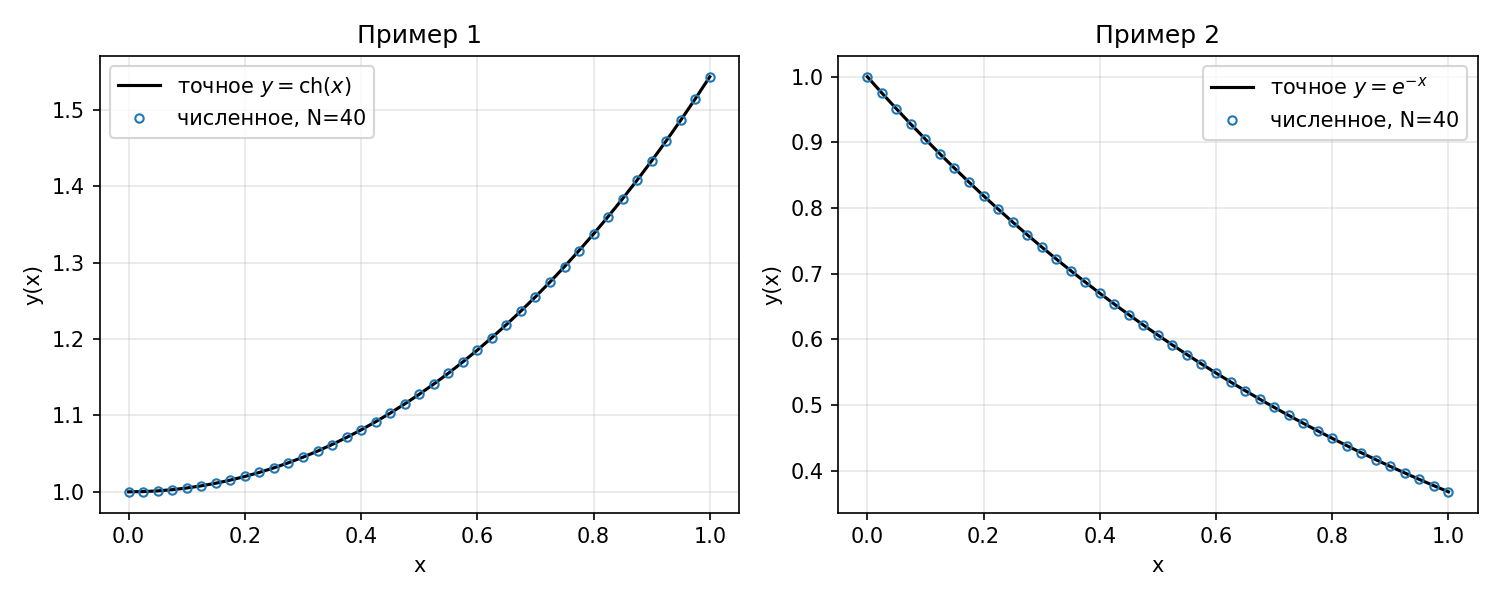
\includegraphics[width=\textwidth]{images/solutions.png}
\caption{Численное (точки) и точное (линия) решения для примеров 1 и 2, $N=40$}
\label{fig:solutions}
\end{figure}

\subsection{Сходимость итерационного процесса}

На рис.~\ref{fig:iter} показана зависимость невязки $\|Y^{(n+1)} - Y^{(n)}\|_\infty$ от номера итерации $n$ в логарифмическом масштабе по оси ординат. Видно, что невязка убывает существенно быстрее любой геометрической прогрессии --- это численное подтверждение факториальной скорости сходимости, обоснованной в разделе~1.2. Требуемая точность $\varepsilon = 10^{-12}$ достигается уже за 8--16 итераций (для $N=40$), независимо от величины $N$.

\begin{figure}[h!]
\centering
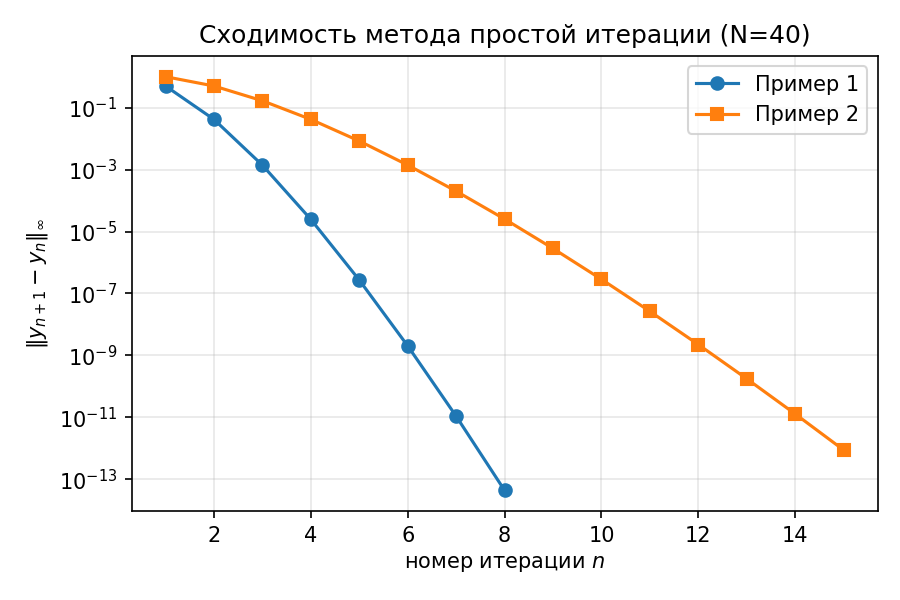
\includegraphics[width=0.75\textwidth]{images/convergence_iterations.png}
\caption{Убывание невязки итерационного процесса по номерам итераций}
\label{fig:iter}
\end{figure}

\subsection{Точность численного решения и порядок сходимости по шагу сетки}

В таблице~\ref{tab:errors} приведены результаты расчётов при $\varepsilon = 10^{-12}$ для последовательности сеток $N = 10, 20, 40, 80, 160$. Погрешность $\Delta_N = \max_i |Y_i - y(x_i)|$ вычислена относительно точного решения; порядок сходимости $p$ оценён по формуле $p = \log_2(\Delta_{N} / \Delta_{2N})$.

\begin{table}[h!]
\centering
\caption{Погрешность численного решения в зависимости от шага сетки}
\label{tab:errors}
\begin{tabular}{|c|c|c|c|c|c|}
\hline
\multirow{2}{*}{$N$} & \multirow{2}{*}{$h$} &
\multicolumn{2}{c|}{Пример 1 ($y=\operatorname{ch}x$)} &
\multicolumn{2}{c|}{Пример 2 ($y=e^{-x}$)} \\
\cline{3-6}
 & & $\Delta_N$ & $p$ & $\Delta_N$ & $p$ \\
\hline
10  & 0.1    & $4.890\times10^{-4}$ & ---   & $3.069\times10^{-4}$ & --- \\
\hline
20  & 0.05   & $1.224\times10^{-4}$ & 2.00  & $7.666\times10^{-5}$ & 2.00 \\
\hline
40  & 0.025  & $3.060\times10^{-5}$ & 2.00  & $1.916\times10^{-5}$ & 2.00 \\
\hline
80  & 0.0125 & $7.651\times10^{-6}$ & 2.00  & $4.790\times10^{-6}$ & 2.00 \\
\hline
160 & 0.00625& $1.913\times10^{-6}$ & 2.00  & $1.198\times10^{-6}$ & 2.00 \\
\hline
\end{tabular}
\end{table}

Число итераций, потребовавшееся для достижения точности $10^{-12}$, составило 8 для примера~1 и 15--16 для примера~2 и практически не зависело от $N$ --- это согласуется с теоретической оценкой факториальной скорости сходимости, не зависящей от дискретизации по $x$.

На рис.~\ref{fig:order} приведена зависимость погрешности $\Delta_N$ от шага сетки $h$ в логарифмических координатах. Экспериментальные точки располагаются на прямой, параллельной прямой $O(h^2)$, что подтверждает теоретический второй порядок точности квадратурной формулы трапеций.

\begin{figure}[h!]
\centering
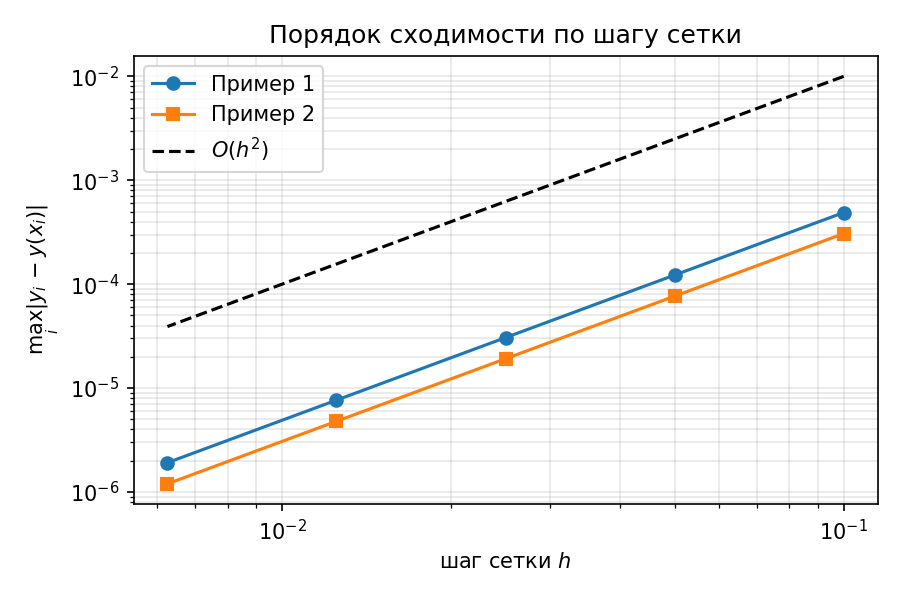
\includegraphics[width=0.75\textwidth]{images/error_vs_h.png}
\caption{Погрешность численного решения в зависимости от шага сетки $h$ (логарифмический масштаб)}
\label{fig:order}
\end{figure}

% ========== ЗАКЛЮЧЕНИЕ ==========
\section*{Заключение}
\addcontentsline{toc}{section}{Заключение}

В курсовом проекте рассмотрен метод простой итерации (метод последовательных приближений) для численного решения линейного интегрального уравнения Вольтерра второго рода. Показано, что в отличие от уравнения Фредгольма второго рода, для уравнения Вольтерра метод сходится безусловно, при любом значении параметра $\lambda$, со скоростью, убывающей быстрее любой геометрической прогрессии (факториальная скорость сходимости).

Построена вычислительная схема, сочетающая метод простой итерации с квадратурной формулой трапеций для дискретизации интеграла, и выполнена её программная реализация на языке Python. На двух тестовых примерах с известными точными решениями ($y=\operatorname{ch}x$ и $y=e^{-x}$) подтверждены:
\begin{itemize}
\item безусловная и быстрая (факториальная) сходимость итерационного процесса --- требуемая точность $10^{-12}$ достигается за 8--16 итераций независимо от числа узлов сетки;
\item второй порядок точности численного решения относительно шага сетки $h$, соответствующий порядку точности использованной квадратурной формулы трапеций.
\end{itemize}

Таким образом, метод простой итерации в сочетании с квадратурными формулами является эффективным и теоретически обоснованным средством численного решения линейных интегральных уравнений Вольтерра второго рода; повышение точности возможно за счёт применения квадратурных формул более высокого порядка (например, формулы Симпсона) без изменения общей схемы метода.

% ========== ЛИТЕРАТУРА ==========
\section*{Список литературы}
\addcontentsline{toc}{section}{Список литературы}

\begin{enumerate}
\item Марчук Г.\,И. Методы вычислительной математики. --- 3-е изд., перераб. и доп. --- М.: Наука, 1989. --- 608~с.
\item Вержбицкий В.\,М. Основы численных методов: учебник для вузов. --- М.: Высшая школа, 2002. --- 840~с.
\item Завьялов Ю.\,С., Квасов Б.\,И., Мирошниченко В.\,Л. Методы сплайн-функций. --- М.: Наука, 1980. --- 352~с.
\item Фаддеев Д.\,К., Фаддеева В.\,Н. Вычислительные методы линейной алгебры. --- 2-е изд. --- М.: Физматгиз, 1963. --- 656~с.
\item Колобов А.\,Г. Численные методы: учебное пособие. --- Владивосток: Изд-во ДВФУ.
\item Бахвалов Н.\,С., Жидков Н.\,П., Кобельков Г.\,М. Численные методы: учебник. --- М.: Лаборатория знаний.
\item Демидович Б.\,П., Марон И.\,А. Основы вычислительной математики. --- М.: Наука, 1970.
\end{enumerate}

\end{document}
